% Created by tikzDevice version 0.12.3.1 on 2023-04-19 11:05:18
% !TEX encoding = UTF-8 Unicode
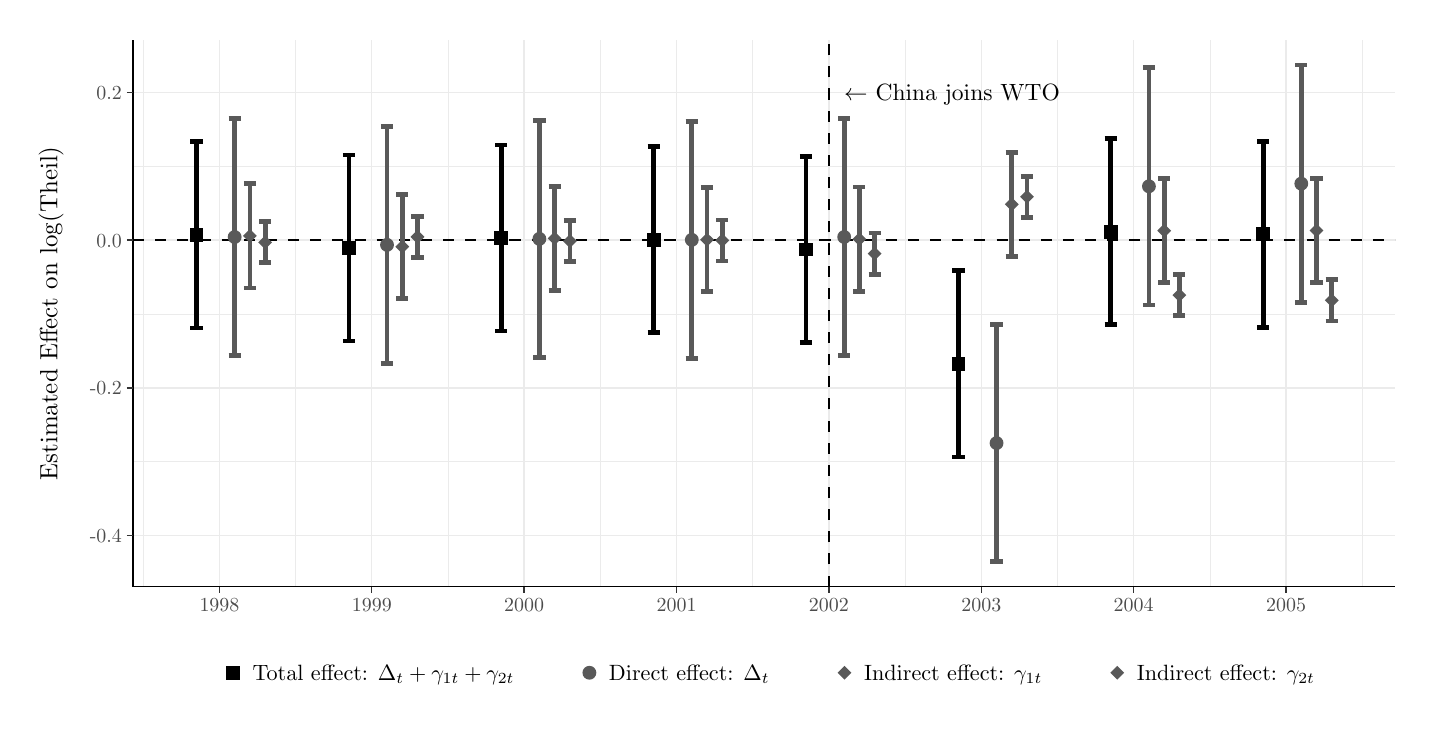
\begin{tikzpicture}[x=1pt,y=1pt]
\definecolor{fillColor}{RGB}{255,255,255}
\path[use as bounding box,fill=fillColor] (0,0) rectangle (498.66,249.33);
\begin{scope}
\path[clip] (  0.00,  0.00) rectangle (498.66,249.33);
\definecolor{drawColor}{RGB}{255,255,255}

\path[draw=drawColor,line width= 0.5pt,line join=round,line cap=round,fill=fillColor] ( -0.00,  0.00) rectangle (498.66,249.33);
\end{scope}
\begin{scope}
\path[clip] ( 38.10, 47.36) rectangle (494.16,244.83);
\definecolor{fillColor}{RGB}{255,255,255}

\path[fill=fillColor] ( 38.10, 47.36) rectangle (494.16,244.83);
\definecolor{drawColor}{gray}{0.92}

\path[draw=drawColor,line width= 0.2pt,line join=round] ( 38.10, 92.50) --
	(494.16, 92.50);

\path[draw=drawColor,line width= 0.2pt,line join=round] ( 38.10,145.87) --
	(494.16,145.87);

\path[draw=drawColor,line width= 0.2pt,line join=round] ( 38.10,199.23) --
	(494.16,199.23);

\path[draw=drawColor,line width= 0.2pt,line join=round] ( 41.76, 47.36) --
	( 41.76,244.83);

\path[draw=drawColor,line width= 0.2pt,line join=round] ( 96.82, 47.36) --
	( 96.82,244.83);

\path[draw=drawColor,line width= 0.2pt,line join=round] (151.88, 47.36) --
	(151.88,244.83);

\path[draw=drawColor,line width= 0.2pt,line join=round] (206.94, 47.36) --
	(206.94,244.83);

\path[draw=drawColor,line width= 0.2pt,line join=round] (262.00, 47.36) --
	(262.00,244.83);

\path[draw=drawColor,line width= 0.2pt,line join=round] (317.06, 47.36) --
	(317.06,244.83);

\path[draw=drawColor,line width= 0.2pt,line join=round] (372.12, 47.36) --
	(372.12,244.83);

\path[draw=drawColor,line width= 0.2pt,line join=round] (427.18, 47.36) --
	(427.18,244.83);

\path[draw=drawColor,line width= 0.2pt,line join=round] (482.24, 47.36) --
	(482.24,244.83);

\path[draw=drawColor,line width= 0.5pt,line join=round] ( 38.10, 65.81) --
	(494.16, 65.81);

\path[draw=drawColor,line width= 0.5pt,line join=round] ( 38.10,119.18) --
	(494.16,119.18);

\path[draw=drawColor,line width= 0.5pt,line join=round] ( 38.10,172.55) --
	(494.16,172.55);

\path[draw=drawColor,line width= 0.5pt,line join=round] ( 38.10,225.92) --
	(494.16,225.92);

\path[draw=drawColor,line width= 0.5pt,line join=round] ( 69.29, 47.36) --
	( 69.29,244.83);

\path[draw=drawColor,line width= 0.5pt,line join=round] (124.35, 47.36) --
	(124.35,244.83);

\path[draw=drawColor,line width= 0.5pt,line join=round] (179.41, 47.36) --
	(179.41,244.83);

\path[draw=drawColor,line width= 0.5pt,line join=round] (234.47, 47.36) --
	(234.47,244.83);

\path[draw=drawColor,line width= 0.5pt,line join=round] (289.53, 47.36) --
	(289.53,244.83);

\path[draw=drawColor,line width= 0.5pt,line join=round] (344.59, 47.36) --
	(344.59,244.83);

\path[draw=drawColor,line width= 0.5pt,line join=round] (399.65, 47.36) --
	(399.65,244.83);

\path[draw=drawColor,line width= 0.5pt,line join=round] (454.71, 47.36) --
	(454.71,244.83);
\definecolor{drawColor}{RGB}{0,0,0}

\path[draw=drawColor,line width= 0.6pt,dash pattern=on 4pt off 4pt ,line join=round] ( 38.10,172.55) -- (494.16,172.55);

\path[draw=drawColor,line width= 0.6pt,dash pattern=on 4pt off 4pt ,line join=round] (289.53, 47.36) -- (289.53,244.83);

\node[text=drawColor,anchor=base west,inner sep=0pt, outer sep=0pt, scale=  0.85] at (295.04,222.98) {$\leftarrow$ China joins WTO};

\path[draw=drawColor,line width= 1.7pt,line join=round] ( 58.83,208.07) --
	( 63.23,208.07);

\path[draw=drawColor,line width= 1.7pt,line join=round] ( 61.03,208.07) --
	( 61.03,140.85);

\path[draw=drawColor,line width= 1.7pt,line join=round] ( 58.83,140.85) --
	( 63.23,140.85);

\path[draw=drawColor,line width= 1.7pt,line join=round] (113.89,203.29) --
	(118.29,203.29);

\path[draw=drawColor,line width= 1.7pt,line join=round] (116.09,203.29) --
	(116.09,136.06);

\path[draw=drawColor,line width= 1.7pt,line join=round] (113.89,136.06) --
	(118.29,136.06);

\path[draw=drawColor,line width= 1.7pt,line join=round] (168.95,206.93) --
	(173.35,206.93);

\path[draw=drawColor,line width= 1.7pt,line join=round] (171.15,206.93) --
	(171.15,139.71);

\path[draw=drawColor,line width= 1.7pt,line join=round] (168.95,139.71) --
	(173.35,139.71);

\path[draw=drawColor,line width= 1.7pt,line join=round] (224.01,206.36) --
	(228.41,206.36);

\path[draw=drawColor,line width= 1.7pt,line join=round] (226.21,206.36) --
	(226.21,139.14);

\path[draw=drawColor,line width= 1.7pt,line join=round] (224.01,139.14) --
	(228.41,139.14);

\path[draw=drawColor,line width= 1.7pt,line join=round] (279.07,202.81) --
	(283.47,202.81);

\path[draw=drawColor,line width= 1.7pt,line join=round] (281.27,202.81) --
	(281.27,135.59);

\path[draw=drawColor,line width= 1.7pt,line join=round] (279.07,135.59) --
	(283.47,135.59);

\path[draw=drawColor,line width= 1.7pt,line join=round] (334.13,161.46) --
	(338.53,161.46);

\path[draw=drawColor,line width= 1.7pt,line join=round] (336.33,161.46) --
	(336.33, 94.24);

\path[draw=drawColor,line width= 1.7pt,line join=round] (334.13, 94.24) --
	(338.53, 94.24);

\path[draw=drawColor,line width= 1.7pt,line join=round] (389.19,209.18) --
	(393.59,209.18);

\path[draw=drawColor,line width= 1.7pt,line join=round] (391.39,209.18) --
	(391.39,141.96);

\path[draw=drawColor,line width= 1.7pt,line join=round] (389.19,141.96) --
	(393.59,141.96);

\path[draw=drawColor,line width= 1.7pt,line join=round] (444.25,208.32) --
	(448.66,208.32);

\path[draw=drawColor,line width= 1.7pt,line join=round] (446.45,208.32) --
	(446.45,141.10);

\path[draw=drawColor,line width= 1.7pt,line join=round] (444.25,141.10) --
	(448.66,141.10);
\definecolor{drawColor}{gray}{0.35}

\path[draw=drawColor,line width= 1.7pt,line join=round] ( 72.59,216.57) --
	( 77.00,216.57);

\path[draw=drawColor,line width= 1.7pt,line join=round] ( 74.79,216.57) --
	( 74.79,130.80);

\path[draw=drawColor,line width= 1.7pt,line join=round] ( 72.59,130.80) --
	( 77.00,130.80);

\path[draw=drawColor,line width= 1.7pt,line join=round] (127.65,213.73) --
	(132.06,213.73);

\path[draw=drawColor,line width= 1.7pt,line join=round] (129.85,213.73) --
	(129.85,127.96);

\path[draw=drawColor,line width= 1.7pt,line join=round] (127.65,127.96) --
	(132.06,127.96);

\path[draw=drawColor,line width= 1.7pt,line join=round] (182.71,215.89) --
	(187.12,215.89);

\path[draw=drawColor,line width= 1.7pt,line join=round] (184.91,215.89) --
	(184.91,130.12);

\path[draw=drawColor,line width= 1.7pt,line join=round] (182.71,130.12) --
	(187.12,130.12);

\path[draw=drawColor,line width= 1.7pt,line join=round] (237.77,215.55) --
	(242.18,215.55);

\path[draw=drawColor,line width= 1.7pt,line join=round] (239.98,215.55) --
	(239.98,129.79);

\path[draw=drawColor,line width= 1.7pt,line join=round] (237.77,129.79) --
	(242.18,129.79);

\path[draw=drawColor,line width= 1.7pt,line join=round] (292.83,216.58) --
	(297.24,216.58);

\path[draw=drawColor,line width= 1.7pt,line join=round] (295.04,216.58) --
	(295.04,130.81);

\path[draw=drawColor,line width= 1.7pt,line join=round] (292.83,130.81) --
	(297.24,130.81);

\path[draw=drawColor,line width= 1.7pt,line join=round] (347.89,142.10) --
	(352.30,142.10);

\path[draw=drawColor,line width= 1.7pt,line join=round] (350.10,142.10) --
	(350.10, 56.34);

\path[draw=drawColor,line width= 1.7pt,line join=round] (347.89, 56.34) --
	(352.30, 56.34);

\path[draw=drawColor,line width= 1.7pt,line join=round] (402.95,234.89) --
	(407.36,234.89);

\path[draw=drawColor,line width= 1.7pt,line join=round] (405.16,234.89) --
	(405.16,149.12);

\path[draw=drawColor,line width= 1.7pt,line join=round] (402.95,149.12) --
	(407.36,149.12);

\path[draw=drawColor,line width= 1.7pt,line join=round] (458.02,235.86) --
	(462.42,235.86);

\path[draw=drawColor,line width= 1.7pt,line join=round] (460.22,235.86) --
	(460.22,150.09);

\path[draw=drawColor,line width= 1.7pt,line join=round] (458.02,150.09) --
	(462.42,150.09);

\path[draw=drawColor,line width= 1.7pt,line join=round] ( 78.10,192.94) --
	( 82.50,192.94);

\path[draw=drawColor,line width= 1.7pt,line join=round] ( 80.30,192.94) --
	( 80.30,155.28);

\path[draw=drawColor,line width= 1.7pt,line join=round] ( 78.10,155.28) --
	( 82.50,155.28);

\path[draw=drawColor,line width= 1.7pt,line join=round] (133.16,189.03) --
	(137.56,189.03);

\path[draw=drawColor,line width= 1.7pt,line join=round] (135.36,189.03) --
	(135.36,151.37);

\path[draw=drawColor,line width= 1.7pt,line join=round] (133.16,151.37) --
	(137.56,151.37);

\path[draw=drawColor,line width= 1.7pt,line join=round] (188.22,192.01) --
	(192.62,192.01);

\path[draw=drawColor,line width= 1.7pt,line join=round] (190.42,192.01) --
	(190.42,154.35);

\path[draw=drawColor,line width= 1.7pt,line join=round] (188.22,154.35) --
	(192.62,154.35);

\path[draw=drawColor,line width= 1.7pt,line join=round] (243.28,191.54) --
	(247.68,191.54);

\path[draw=drawColor,line width= 1.7pt,line join=round] (245.48,191.54) --
	(245.48,153.89);

\path[draw=drawColor,line width= 1.7pt,line join=round] (243.28,153.89) --
	(247.68,153.89);

\path[draw=drawColor,line width= 1.7pt,line join=round] (298.34,191.77) --
	(302.74,191.77);

\path[draw=drawColor,line width= 1.7pt,line join=round] (300.54,191.77) --
	(300.54,154.11);

\path[draw=drawColor,line width= 1.7pt,line join=round] (298.34,154.11) --
	(302.74,154.11);

\path[draw=drawColor,line width= 1.7pt,line join=round] (353.40,204.32) --
	(357.81,204.32);

\path[draw=drawColor,line width= 1.7pt,line join=round] (355.60,204.32) --
	(355.60,166.67);

\path[draw=drawColor,line width= 1.7pt,line join=round] (353.40,166.67) --
	(357.81,166.67);

\path[draw=drawColor,line width= 1.7pt,line join=round] (408.46,194.79) --
	(412.87,194.79);

\path[draw=drawColor,line width= 1.7pt,line join=round] (410.66,194.79) --
	(410.66,157.13);

\path[draw=drawColor,line width= 1.7pt,line join=round] (408.46,157.13) --
	(412.87,157.13);

\path[draw=drawColor,line width= 1.7pt,line join=round] (463.52,194.87) --
	(467.93,194.87);

\path[draw=drawColor,line width= 1.7pt,line join=round] (465.72,194.87) --
	(465.72,157.21);

\path[draw=drawColor,line width= 1.7pt,line join=round] (463.52,157.21) --
	(467.93,157.21);

\path[draw=drawColor,line width= 1.7pt,line join=round] ( 83.60,179.18) --
	( 88.01,179.18);

\path[draw=drawColor,line width= 1.7pt,line join=round] ( 85.81,179.18) --
	( 85.81,164.35);

\path[draw=drawColor,line width= 1.7pt,line join=round] ( 83.60,164.35) --
	( 88.01,164.35);

\path[draw=drawColor,line width= 1.7pt,line join=round] (138.66,181.15) --
	(143.07,181.15);

\path[draw=drawColor,line width= 1.7pt,line join=round] (140.87,181.15) --
	(140.87,166.31);

\path[draw=drawColor,line width= 1.7pt,line join=round] (138.66,166.31) --
	(143.07,166.31);

\path[draw=drawColor,line width= 1.7pt,line join=round] (193.72,179.65) --
	(198.13,179.65);

\path[draw=drawColor,line width= 1.7pt,line join=round] (195.93,179.65) --
	(195.93,164.82);

\path[draw=drawColor,line width= 1.7pt,line join=round] (193.72,164.82) --
	(198.13,164.82);

\path[draw=drawColor,line width= 1.7pt,line join=round] (248.78,179.88) --
	(253.19,179.88);

\path[draw=drawColor,line width= 1.7pt,line join=round] (250.99,179.88) --
	(250.99,165.05);

\path[draw=drawColor,line width= 1.7pt,line join=round] (248.78,165.05) --
	(253.19,165.05);

\path[draw=drawColor,line width= 1.7pt,line join=round] (303.85,175.09) --
	(308.25,175.09);

\path[draw=drawColor,line width= 1.7pt,line join=round] (306.05,175.09) --
	(306.05,160.26);

\path[draw=drawColor,line width= 1.7pt,line join=round] (303.85,160.26) --
	(308.25,160.26);

\path[draw=drawColor,line width= 1.7pt,line join=round] (358.91,195.65) --
	(363.31,195.65);

\path[draw=drawColor,line width= 1.7pt,line join=round] (361.11,195.65) --
	(361.11,180.82);

\path[draw=drawColor,line width= 1.7pt,line join=round] (358.91,180.82) --
	(363.31,180.82);

\path[draw=drawColor,line width= 1.7pt,line join=round] (413.97,160.12) --
	(418.37,160.12);

\path[draw=drawColor,line width= 1.7pt,line join=round] (416.17,160.12) --
	(416.17,145.29);

\path[draw=drawColor,line width= 1.7pt,line join=round] (413.97,145.29) --
	(418.37,145.29);

\path[draw=drawColor,line width= 1.7pt,line join=round] (469.03,158.21) --
	(473.43,158.21);

\path[draw=drawColor,line width= 1.7pt,line join=round] (471.23,158.21) --
	(471.23,143.38);

\path[draw=drawColor,line width= 1.7pt,line join=round] (469.03,143.38) --
	(473.43,143.38);
\definecolor{fillColor}{RGB}{0,0,0}

\path[fill=fillColor] ( 58.53,171.96) --
	( 63.53,171.96) --
	( 63.53,176.96) --
	( 58.53,176.96) --
	cycle;

\path[fill=fillColor] (113.59,167.18) --
	(118.59,167.18) --
	(118.59,172.17) --
	(113.59,172.17) --
	cycle;

\path[fill=fillColor] (168.65,170.82) --
	(173.65,170.82) --
	(173.65,175.82) --
	(168.65,175.82) --
	cycle;

\path[fill=fillColor] (223.71,170.25) --
	(228.71,170.25) --
	(228.71,175.25) --
	(223.71,175.25) --
	cycle;

\path[fill=fillColor] (278.77,166.71) --
	(283.77,166.71) --
	(283.77,171.70) --
	(278.77,171.70) --
	cycle;

\path[fill=fillColor] (333.83,125.35) --
	(338.83,125.35) --
	(338.83,130.35) --
	(333.83,130.35) --
	cycle;

\path[fill=fillColor] (388.89,173.07) --
	(393.89,173.07) --
	(393.89,178.07) --
	(388.89,178.07) --
	cycle;

\path[fill=fillColor] (443.96,172.21) --
	(448.95,172.21) --
	(448.95,177.21) --
	(443.96,177.21) --
	cycle;
\definecolor{fillColor}{gray}{0.35}

\path[fill=fillColor] ( 74.79,173.68) circle (  2.50);

\path[fill=fillColor] (129.85,170.85) circle (  2.50);

\path[fill=fillColor] (184.91,173.01) circle (  2.50);

\path[fill=fillColor] (239.98,172.67) circle (  2.50);

\path[fill=fillColor] (295.04,173.69) circle (  2.50);

\path[fill=fillColor] (350.10, 99.22) circle (  2.50);

\path[fill=fillColor] (405.16,192.01) circle (  2.50);

\path[fill=fillColor] (460.22,192.97) circle (  2.50);

\path[fill=fillColor] ( 77.80,174.11) --
	( 80.30,176.61) --
	( 82.80,174.11) --
	( 80.30,171.61) --
	cycle;

\path[fill=fillColor] (132.86,170.20) --
	(135.36,172.70) --
	(137.86,170.20) --
	(135.36,167.70) --
	cycle;

\path[fill=fillColor] (187.92,173.18) --
	(190.42,175.68) --
	(192.92,173.18) --
	(190.42,170.68) --
	cycle;

\path[fill=fillColor] (242.98,172.72) --
	(245.48,175.21) --
	(247.98,172.72) --
	(245.48,170.22) --
	cycle;

\path[fill=fillColor] (298.04,172.94) --
	(300.54,175.44) --
	(303.04,172.94) --
	(300.54,170.44) --
	cycle;

\path[fill=fillColor] (353.11,185.50) --
	(355.60,187.99) --
	(358.10,185.50) --
	(355.60,183.00) --
	cycle;

\path[fill=fillColor] (408.17,175.96) --
	(410.66,178.46) --
	(413.16,175.96) --
	(410.66,173.46) --
	cycle;

\path[fill=fillColor] (463.23,176.04) --
	(465.72,178.54) --
	(468.22,176.04) --
	(465.72,173.54) --
	cycle;

\path[fill=fillColor] ( 83.31,171.77) --
	( 85.81,174.26) --
	( 88.30,171.77) --
	( 85.81,169.27) --
	cycle;

\path[fill=fillColor] (138.37,173.73) --
	(140.87,176.23) --
	(143.36,173.73) --
	(140.87,171.23) --
	cycle;

\path[fill=fillColor] (193.43,172.23) --
	(195.93,174.73) --
	(198.42,172.23) --
	(195.93,169.74) --
	cycle;

\path[fill=fillColor] (248.49,172.47) --
	(250.99,174.97) --
	(253.49,172.47) --
	(250.99,169.97) --
	cycle;

\path[fill=fillColor] (303.55,167.67) --
	(306.05,170.17) --
	(308.55,167.67) --
	(306.05,165.18) --
	cycle;

\path[fill=fillColor] (358.61,188.23) --
	(361.11,190.73) --
	(363.61,188.23) --
	(361.11,185.74) --
	cycle;

\path[fill=fillColor] (413.67,152.70) --
	(416.17,155.20) --
	(418.67,152.70) --
	(416.17,150.20) --
	cycle;

\path[fill=fillColor] (468.73,150.80) --
	(471.23,153.29) --
	(473.73,150.80) --
	(471.23,148.30) --
	cycle;
\end{scope}
\begin{scope}
\path[clip] (  0.00,  0.00) rectangle (498.66,249.33);
\definecolor{drawColor}{RGB}{0,0,0}

\path[draw=drawColor,line width= 0.5pt,line join=round] ( 38.10, 47.36) --
	( 38.10,244.83);
\end{scope}
\begin{scope}
\path[clip] (  0.00,  0.00) rectangle (498.66,249.33);
\definecolor{drawColor}{gray}{0.30}

\node[text=drawColor,anchor=base east,inner sep=0pt, outer sep=0pt, scale=  0.72] at ( 34.05, 63.33) {-0.4};

\node[text=drawColor,anchor=base east,inner sep=0pt, outer sep=0pt, scale=  0.72] at ( 34.05,116.70) {-0.2};

\node[text=drawColor,anchor=base east,inner sep=0pt, outer sep=0pt, scale=  0.72] at ( 34.05,170.07) {0.0};

\node[text=drawColor,anchor=base east,inner sep=0pt, outer sep=0pt, scale=  0.72] at ( 34.05,223.44) {0.2};
\end{scope}
\begin{scope}
\path[clip] (  0.00,  0.00) rectangle (498.66,249.33);
\definecolor{drawColor}{gray}{0.20}

\path[draw=drawColor,line width= 0.5pt,line join=round] ( 35.85, 65.81) --
	( 38.10, 65.81);

\path[draw=drawColor,line width= 0.5pt,line join=round] ( 35.85,119.18) --
	( 38.10,119.18);

\path[draw=drawColor,line width= 0.5pt,line join=round] ( 35.85,172.55) --
	( 38.10,172.55);

\path[draw=drawColor,line width= 0.5pt,line join=round] ( 35.85,225.92) --
	( 38.10,225.92);
\end{scope}
\begin{scope}
\path[clip] (  0.00,  0.00) rectangle (498.66,249.33);
\definecolor{drawColor}{RGB}{0,0,0}

\path[draw=drawColor,line width= 0.5pt,line join=round] ( 38.10, 47.36) --
	(494.16, 47.36);
\end{scope}
\begin{scope}
\path[clip] (  0.00,  0.00) rectangle (498.66,249.33);
\definecolor{drawColor}{gray}{0.20}

\path[draw=drawColor,line width= 0.5pt,line join=round] ( 69.29, 45.11) --
	( 69.29, 47.36);

\path[draw=drawColor,line width= 0.5pt,line join=round] (124.35, 45.11) --
	(124.35, 47.36);

\path[draw=drawColor,line width= 0.5pt,line join=round] (179.41, 45.11) --
	(179.41, 47.36);

\path[draw=drawColor,line width= 0.5pt,line join=round] (234.47, 45.11) --
	(234.47, 47.36);

\path[draw=drawColor,line width= 0.5pt,line join=round] (289.53, 45.11) --
	(289.53, 47.36);

\path[draw=drawColor,line width= 0.5pt,line join=round] (344.59, 45.11) --
	(344.59, 47.36);

\path[draw=drawColor,line width= 0.5pt,line join=round] (399.65, 45.11) --
	(399.65, 47.36);

\path[draw=drawColor,line width= 0.5pt,line join=round] (454.71, 45.11) --
	(454.71, 47.36);
\end{scope}
\begin{scope}
\path[clip] (  0.00,  0.00) rectangle (498.66,249.33);
\definecolor{drawColor}{gray}{0.30}

\node[text=drawColor,anchor=base,inner sep=0pt, outer sep=0pt, scale=  0.72] at ( 69.29, 38.35) {1998};

\node[text=drawColor,anchor=base,inner sep=0pt, outer sep=0pt, scale=  0.72] at (124.35, 38.35) {1999};

\node[text=drawColor,anchor=base,inner sep=0pt, outer sep=0pt, scale=  0.72] at (179.41, 38.35) {2000};

\node[text=drawColor,anchor=base,inner sep=0pt, outer sep=0pt, scale=  0.72] at (234.47, 38.35) {2001};

\node[text=drawColor,anchor=base,inner sep=0pt, outer sep=0pt, scale=  0.72] at (289.53, 38.35) {2002};

\node[text=drawColor,anchor=base,inner sep=0pt, outer sep=0pt, scale=  0.72] at (344.59, 38.35) {2003};

\node[text=drawColor,anchor=base,inner sep=0pt, outer sep=0pt, scale=  0.72] at (399.65, 38.35) {2004};

\node[text=drawColor,anchor=base,inner sep=0pt, outer sep=0pt, scale=  0.72] at (454.71, 38.35) {2005};
\end{scope}
\begin{scope}
\path[clip] (  0.00,  0.00) rectangle (498.66,249.33);
\definecolor{drawColor}{RGB}{0,0,0}

\node[text=drawColor,rotate= 90.00,anchor=base,inner sep=0pt, outer sep=0pt, scale=  0.90] at ( 10.70,146.10) {Estimated Effect on $\log($Theil$)$};
\end{scope}
\begin{scope}
\path[clip] (  0.00,  0.00) rectangle (498.66,249.33);
\definecolor{fillColor}{RGB}{255,255,255}

\path[fill=fillColor] ( 52.61,  4.50) rectangle (479.65, 27.95);
\end{scope}
\begin{scope}
\path[clip] (  0.00,  0.00) rectangle (498.66,249.33);
\definecolor{fillColor}{RGB}{255,255,255}

\path[fill=fillColor] ( 59.96,  9.00) rectangle ( 88.41, 23.45);
\end{scope}
\begin{scope}
\path[clip] (  0.00,  0.00) rectangle (498.66,249.33);
\definecolor{fillColor}{RGB}{0,0,0}

\path[fill=fillColor] ( 71.68, 13.73) --
	( 76.68, 13.73) --
	( 76.68, 18.72) --
	( 71.68, 18.72) --
	cycle;
\end{scope}
\begin{scope}
\path[clip] (  0.00,  0.00) rectangle (498.66,249.33);
\definecolor{fillColor}{RGB}{255,255,255}

\path[fill=fillColor] (188.76,  9.00) rectangle (217.21, 23.45);
\end{scope}
\begin{scope}
\path[clip] (  0.00,  0.00) rectangle (498.66,249.33);
\definecolor{fillColor}{gray}{0.35}

\path[fill=fillColor] (202.98, 16.23) circle (  2.50);
\end{scope}
\begin{scope}
\path[clip] (  0.00,  0.00) rectangle (498.66,249.33);
\definecolor{fillColor}{RGB}{255,255,255}

\path[fill=fillColor] (280.95,  9.00) rectangle (309.40, 23.45);
\end{scope}
\begin{scope}
\path[clip] (  0.00,  0.00) rectangle (498.66,249.33);
\definecolor{fillColor}{gray}{0.35}

\path[fill=fillColor] (292.68, 16.23) --
	(295.17, 18.72) --
	(297.67, 16.23) --
	(295.17, 13.73) --
	cycle;
\end{scope}
\begin{scope}
\path[clip] (  0.00,  0.00) rectangle (498.66,249.33);
\definecolor{fillColor}{RGB}{255,255,255}

\path[fill=fillColor] (379.47,  9.00) rectangle (407.92, 23.45);
\end{scope}
\begin{scope}
\path[clip] (  0.00,  0.00) rectangle (498.66,249.33);
\definecolor{fillColor}{gray}{0.35}

\path[fill=fillColor] (391.20, 16.23) --
	(393.70, 18.72) --
	(396.19, 16.23) --
	(393.70, 13.73) --
	cycle;
\end{scope}
\begin{scope}
\path[clip] (  0.00,  0.00) rectangle (498.66,249.33);
\definecolor{drawColor}{RGB}{0,0,0}

\node[text=drawColor,anchor=base west,inner sep=0pt, outer sep=0pt, scale=  0.80] at ( 81.25, 13.47) {Total effect: $\Delta_t + \gamma_{1t} + \gamma_{2t}$};
\end{scope}
\begin{scope}
\path[clip] (  0.00,  0.00) rectangle (498.66,249.33);
\definecolor{drawColor}{RGB}{0,0,0}

\node[text=drawColor,anchor=base west,inner sep=0pt, outer sep=0pt, scale=  0.80] at (210.05, 13.47) {Direct effect: $\Delta_t$};
\end{scope}
\begin{scope}
\path[clip] (  0.00,  0.00) rectangle (498.66,249.33);
\definecolor{drawColor}{RGB}{0,0,0}

\node[text=drawColor,anchor=base west,inner sep=0pt, outer sep=0pt, scale=  0.80] at (302.25, 13.47) {Indirect effect: $\gamma_{1t}$};
\end{scope}
\begin{scope}
\path[clip] (  0.00,  0.00) rectangle (498.66,249.33);
\definecolor{drawColor}{RGB}{0,0,0}

\node[text=drawColor,anchor=base west,inner sep=0pt, outer sep=0pt, scale=  0.80] at (400.77, 13.47) {Indirect effect: $\gamma_{2t}$};
\end{scope}
\end{tikzpicture}
